%%%%%%%%%%%%%%%%%%%%%%%%%%%%%%%%%%%%%%%%%
% Original author:
% Linux and Unix Users Group at Virginia Tech Wiki
% (https://vtluug.org/wiki/Example_LaTeX_chem_lab_report)
% Modified by: Hector F. Jimenez S, for general Reports.
% License:
% CC BY-NC-SA 3.0 
%%%%%%%%%%%%%%%%%%%%%%%%%%%%%%%%%%%%%%%%%
%----------------------------------------
%	PACKAGES AND DOCUMENT CONFIGURATIONS
%---------------------------------------
\documentclass[paper=a4, fontsize=12pt]{article} 		% A4 paper and 11pt font size
\usepackage[T1]{fontenc} 								% Use 8-bit encoding that has 256 glyphs
%\usepackage{fourier}		 							% Use the Adobe Utopia font for the document 
\usepackage[spanish,english]{babel}						% Spanish Language, templates uses some sections in english.
\selectlanguage{spanish}								% main language.
\usepackage{subfig}
\usepackage{multirow}
\PassOptionsToPackage{spanish}{babel}
\renewcommand{\figurename}{Figura}						% Force rename of figure.
\renewcommand{\figurename}{Fig.}
\usepackage[figurename=Fig.]{caption}
\usepackage[utf8]{inputenc}								% tildes for spanish language.
\usepackage{amsmath,amsfonts,amsthm} 					% Math packages.
\usepackage{minted}										% For syntax highlighting.
	    \renewcommand\listingscaption{Código}			%rename the source code minted !
\usepackage{float}										% Image will be in the same place as you want.!!! x-/
\usepackage{sectsty} 									% Allows customizing section commands
\allsectionsfont{\centering \normalfont\scshape}	   	% Make all sections centered, the default font and small caps
\usepackage{hyperref}
\hypersetup{											%Setups the false color and borders.
    colorlinks=false,
    pdfborder={0 0 0},
}
\newcommand\fnurl[2]{%									% set a simple and quick footnote command and include url.
\href{#2}{#1}\footnote{\url{#2}}%	
}
\usepackage{graphicx}									% Import easyly images.
\graphicspath{ {./images/} }							% Where to look for the images.
\DeclareGraphicsExtensions{.pdf,.png,.jpg}				% Graphics Extension to be used
\usepackage[notes,backend=biber]{biblatex-chicago}		% Bibliography and references.
\bibliography{biblio}									% bibliography filename.
\usepackage{fancyhdr} 									% Custom headers and footers
\pagestyle{fancyplain} 									% Makes all pages in the document conform to the custom headers and footers
\fancyhead{} 											% No page header
\fancyfoot[L]{} 										% Empty left footer
\fancyfoot[C]{} 										% Empty center footer
\fancyfoot[R]{\thepage} 								% Page numbering for right footer
\renewcommand{\headrulewidth}{0pt} 						% Remove header underlines
\renewcommand{\footrulewidth}{0pt} 						% Remove footer underlines
\setlength{\headheight}{13.6pt} 					    % Customize the height of the header
\numberwithin{equation}{section}						% Number equations within sections (i.e. 1.1, 1.2, 2.1, 2.2 instead of 1, 2, 3, 4)
%\numberwithin{figure}{section} 						% Number figures within sections (i.e. 1.1, 1.2, 2.1, 2.2 instead of 1, 2)
\numberwithin{table}{section} 							% Number tables within sections (i.e. 1.1, 1.2, 2.1, 2.2 instead of 1, 2, 3, 4)
\setlength\parindent{0pt} 								% Removes all indentation from paragraphs
\newcommand{\horrule}[1]{\rule{\linewidth}{#1}} 		% Create horizontal rule command with 1 argument of height
\usepackage{listings}% http://ctan.org/pkg/listings
\usepackage{multicol}
\usepackage{caption}
\usepackage{subfig}
\renewcommand{\lstlistingname}{Código}	
\title{Sistemas Operativos I\\ 
\horrule{0.5pt} \\[0.4cm] 								% Thin top horizontal rule	Title rule
\textit{Taller 10: Caso de estudio del sistema operativo Windows Server 2003}
\horrule{1pt} \\[0.5cm] 			
} 			
\author{												
Héctor F. \textsc{Jiménez Saldarriaga.}\\				% Authors begin.
\texttt{hfjimenez@utp.edu.co} \\						
\texttt{PGP KEY ID: 0xB05AD7B8}
} 
% End of  Author name
\date{}    						                       % Date for the report, this will hide the \today.
\begin{document}
\maketitle                      			           % Insert the title, author and date
\begin{center}
\begin{tabular}{l r}								   % two column to
Fecha de Entrega: & Mayo, 2018 \\				   	   % Profesor Details.
Profesor: & Cesar Manuel Castillo Rodriguez
\end{tabular}
\end{center}
%%%%%%%%%%%	
% Let's start the document.
%%%%%%%%%%%	
\section{Objetivos}
\begin{itemize}
	\item Evolución
	\item Realizar el proceso de instalación del sistema operativo	
    \item Identificar el manejo de Archivos, Shell
    \item Estructura del Sistema Operativo
    \item Clasificación del Sistema Operativo
\end{itemize}
\section{Evolución de Windows Server 2003} 
Windows Server 2003 es un sistema operativo de la familia Windows desarrollado por la empresa Microsoft para servidores, esta empresa libero esta versión en el mercado el 24 de abril de 2003(véase la figura \ref{fig:mejora}). Está basada en tecnología NT y versión del núcleo NT 5.2. En términos generales, Windows Server 2003 se podría considerar como un Windows XP modificado para labores empresariales, que permita realizar mas labores empresariales,  su enfoque es principalmente en la mejora de rendimiento mejor uso de recursos de hardware, mejora en los usos del procesador para atender múltiples tareas y usuarios concurrentes dentro de las empresa y organizaciones de mediano y gran tamaño.

Windows Server 2003 en su ultima versión tiene la actualización R2, liberada en diciembre de 2005. Su sucesor es el sistema operativo Windows Server 2008, el cual tiene muchas bases de desarrollo del kernel de Windows vista y caracteristicas de Windows Server 2003.
Algunas de las aplicaciones que ofrece son mayormente usadas en un Windows Server 2003 son: 
\begin{itemize}
  \item Servidor de archivos
  \item Servidor de impresiones
  \item Servidor de aplicaciones
  \item Servidor de correo (SMTP/POP)
  \item Servidor de terminal
  \item Servidor de Redes privadas virtuales (VPN) (o acceso remoto al servidor)
  \item Controlador de Dominios (mediante Active Directory)
  \item Servidor DNS
  \item Servidor DHCP
  \item Servidor de Streaming de Vídeo
  \item Servidor WINS
  \item Servidor RIS Remote Installation Services (Servicios de instalación remota)
\end{itemize}
\subsection{Mejoras respecto a Windows 2000 Server}
Se puede encontrar algunas diferencias entre  Windows server 2000 y Windows Server 2003 \fnurl{aqui}{https://blogs.technet.microsoft.com/perfguru/2008/03/07/differences-between-windows-server-2000-and-windows-server-2003-print-clusters-and-their-registry-structure/} pero principalmente son:
\begin{enumerate}
\item Durante la instalación arranca con el mínimo de servicios activados para no comprometer la seguridad del sistema
\item Mejoras en el manejo de políticas de seguridad
\item Active Directory ya no utiliza NetBIOS sino que es necesaria la presencia de un DNS que soporte Service Records (detección de servicios ofrecidos por una máquina a través de un DNS)
\item Soporte para nuevas versiones de IIS.
\item Drivers y administrador del servidor de impresiones es mucho mas sencilla para los clientes.
\end{enumerate}
A continuacion se puede observar un timeline de las versiones de Windows Server y la relación de ellas en desarrollo.
\begin{center}
\begin{figure}[H]
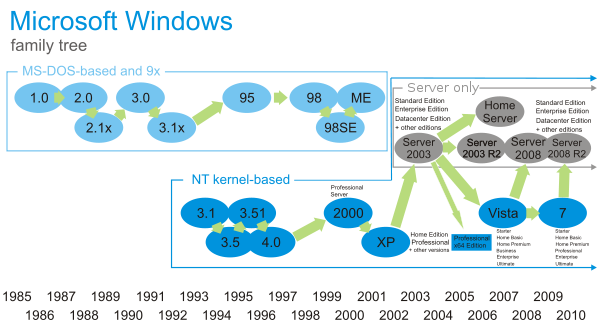
\includegraphics[scale=0.6]{imgs/diff.png}
\caption{Timeline, Microsoft Windows. Sistemas Operativos y relación de Kernels}
\label{fig:mejora}
\end{figure}
\end{center}

\section{Proceso de instalación Windows Server 2003}
El proceso para realizar la instalación de este sistema operativo es muy similar a el de realizar la instalacion de un Windows XP SP3, para ello es necesario descargar el paquete que contiene la imagen ISO con la licencia correspondiente. Para esta maquina virtual se establecen dos cores de procesador, 2GB de memoria RAM y 3 tarjetas de red para probar el  manejo de interfaces de red.
\begin{figure}[H]
 	\centering
   	\subfloat[Bienvenida Instalador Windows Server]{\label{fig:bienvenida}{
   		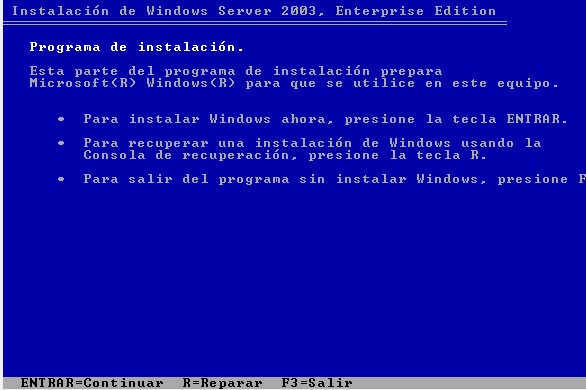
\includegraphics[width=0.68\textwidth]{imgs/2.png}
   		}}
	\subfloat[Terminos y condiciones Windows Server]{\label{fig:formateada}{
   		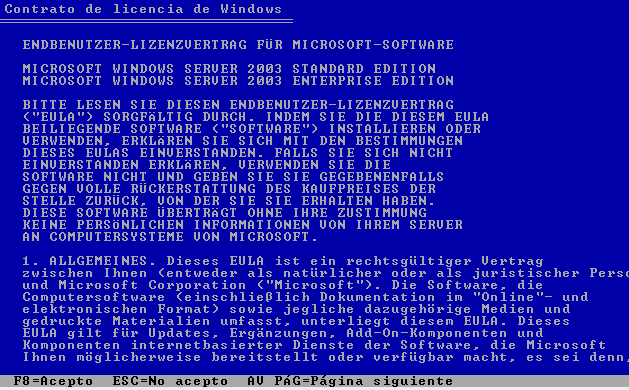
\includegraphics[width=0.68\textwidth]{imgs/3.png}
        }}
       \hfill
	\subfloat[Seleccionamos el disco duro en el que instalaremos el Sistema.]{\label{fig:disco}{
   		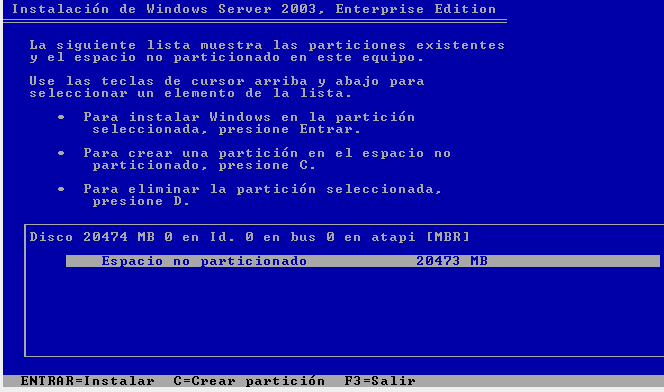
\includegraphics[width=0.68\textwidth]{imgs/4.png}
        }}
	\subfloat[Creamos las particiones correspondientes, 2 una como C: y otra para data D:]{\label{fig:particion}{
   		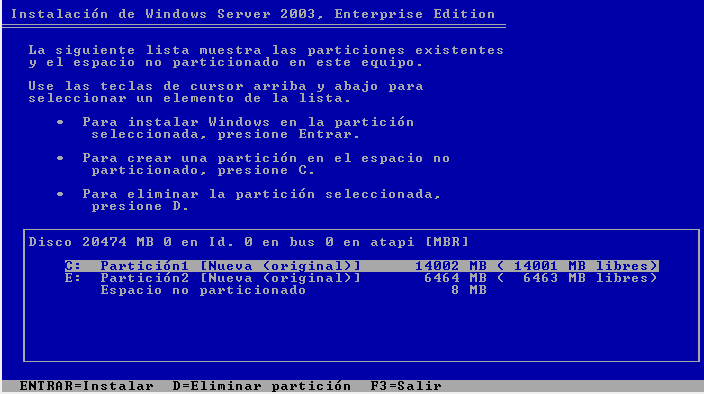
\includegraphics[width=0.68\textwidth]{imgs/5.png}
        }}
        \hfill
	\subfloat[Dado que el disco esta limpio usamos la opción rápida]{\label{fig:particiones}{
   		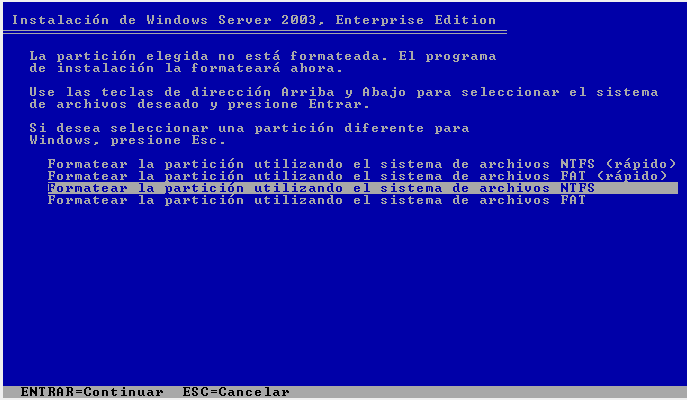
\includegraphics[width=0.68\textwidth]{imgs/6.png}
        }}
	\subfloat[Formateo de disco en progreso]{\label{fig:iniciado}{
   		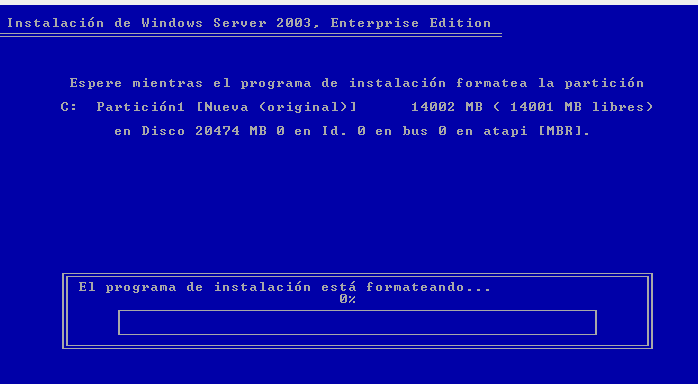
\includegraphics[width=0.68\textwidth]{imgs/7.png}
        }}
	\caption{Configuración inicial de instalación}
\end{figure}

\begin{figure}[H]
 	\centering
   	\subfloat[Progreso de Formateado de particiones]{\label{fig:bienvenida}{
   		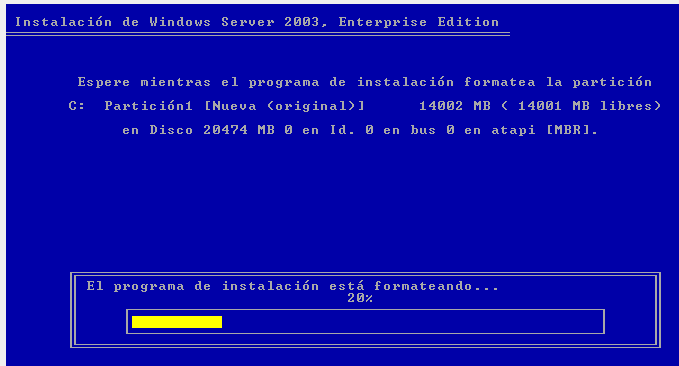
\includegraphics[width=0.68\textwidth]{imgs/8.png}
   		}}
	\subfloat[Progreso de instalación, copia de archivos]{\label{fig:insta1}{
   		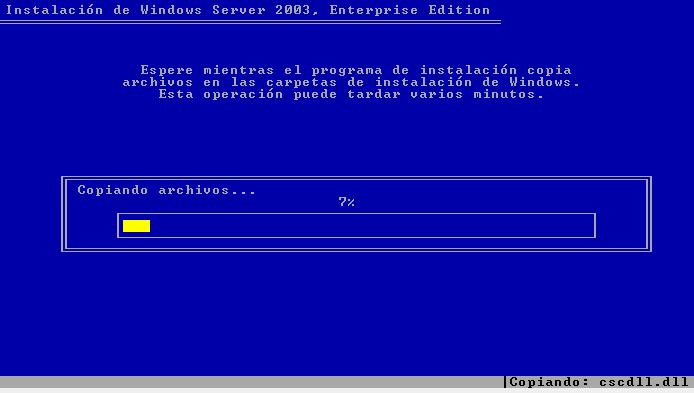
\includegraphics[width=0.68\textwidth]{imgs/9.png}
        }}
       \hfill
	\subfloat[Progreso de instalación, copia de archivos]{\label{fig:insta}{
   		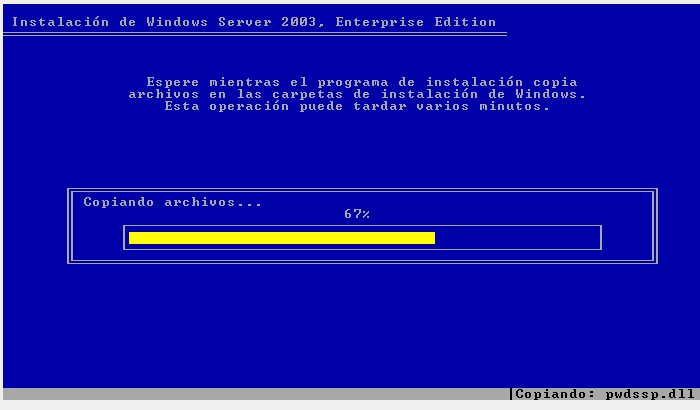
\includegraphics[width=0.68\textwidth]{imgs/10.png}
        }}
      \subfloat[Finaliza la instalacion del sistema base de Windows Server.]{\label{fig:ufs}{
   		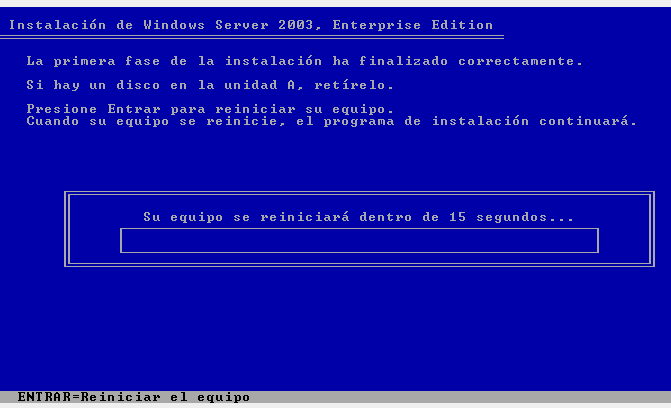
\includegraphics[width=0.68\textwidth]{imgs/11.png}
        }}
        \hfill
	\subfloat[Inicio de Sistema Base Windows Server]{\label{fig:inicianbase}{
   		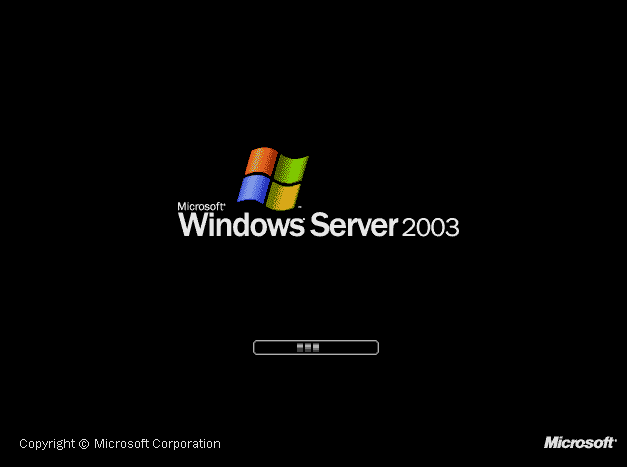
\includegraphics[width=0.68\textwidth]{imgs/12.png}
        }}
      \subfloat[Install Wizard gráfico iniciado.]{\label{fig:wizard}{
   		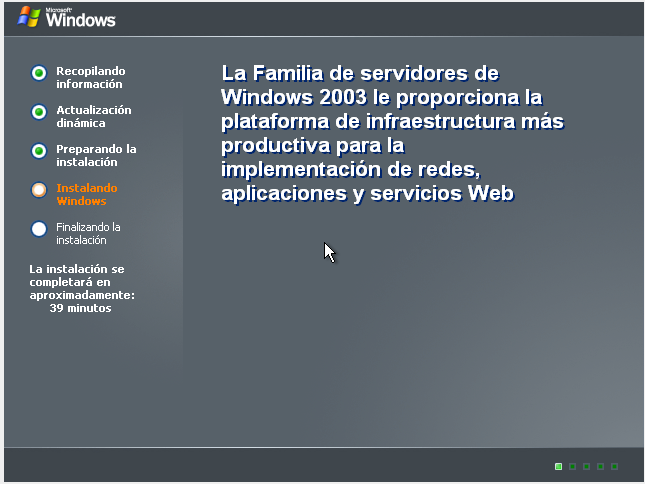
\includegraphics[width=0.68\textwidth]{imgs/13.png}
        }}
	\caption{Proceso secuencial de instalación, Windows Server 2003}
\end{figure}

\begin{figure}[H]
 	\centering
   	\subfloat[Algunas Características de Windows Server 2003]{\label{fig:bienvenida}{
   		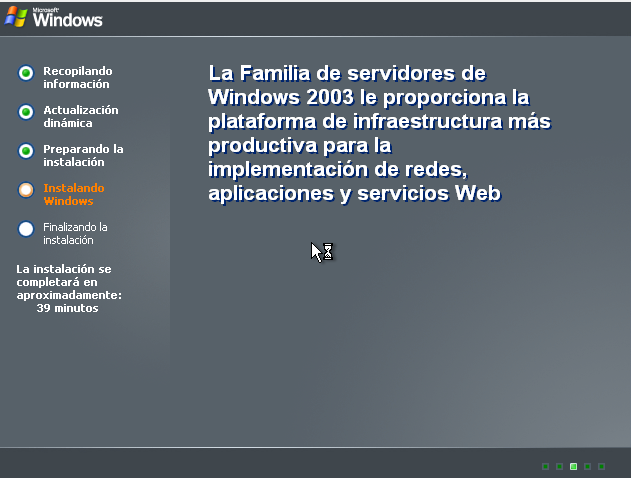
\includegraphics[width=0.68\textwidth]{imgs/15.png}
   		}}
	\subfloat[Configuracion de Cuenta, organización]{\label{fig:cuenta}{
   		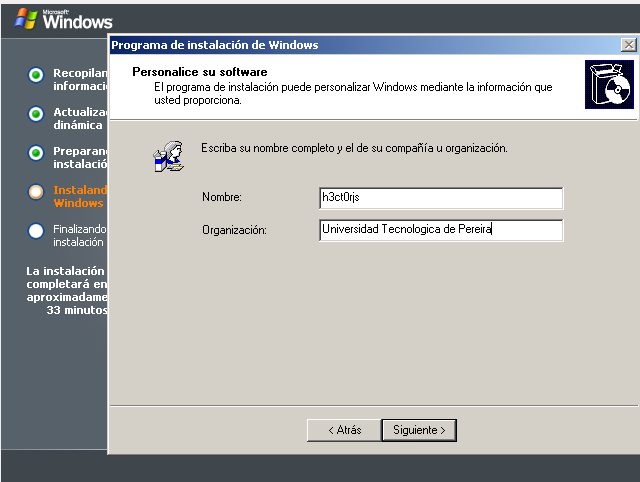
\includegraphics[width=0.68\textwidth]{imgs/16.png}
        }}
       \hfill
	\subfloat[Serial y Licencia producto]{\label{fig:serial}{
   		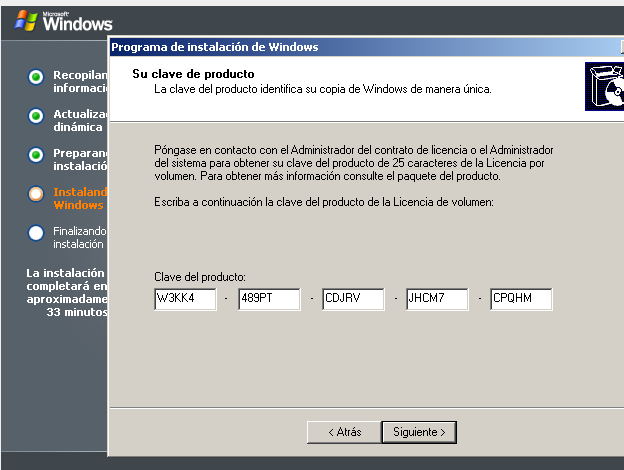
\includegraphics[width=0.68\textwidth]{imgs/17.png}
        }}
      \subfloat[Configuracion Horaria.]{\label{fig:hora}{
   		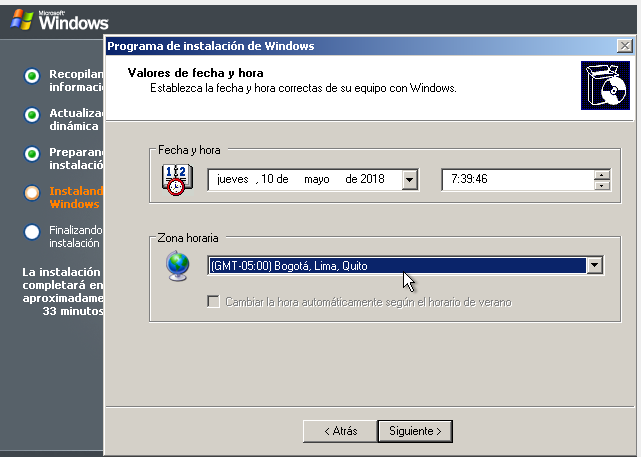
\includegraphics[width=0.68\textwidth]{imgs/18.png}
        }}
        \hfill
	\subfloat[Configuración de Red]{\label{fig:red}{
   		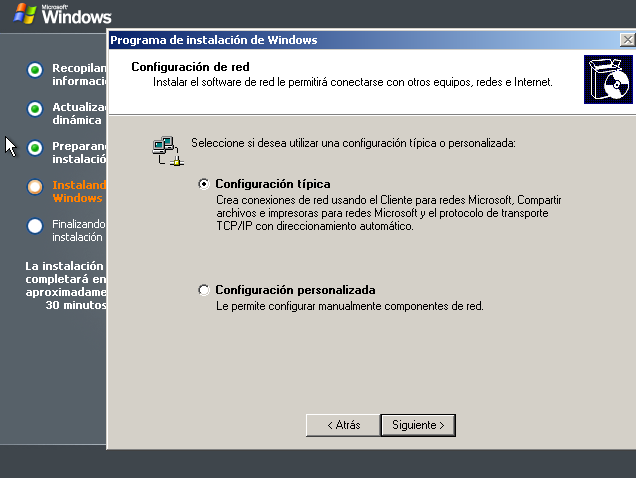
\includegraphics[width=0.68\textwidth]{imgs/19.png}
        }}
      \subfloat[ Establecimiento de nombre de dominio red]{\label{fig:ufs}{
   		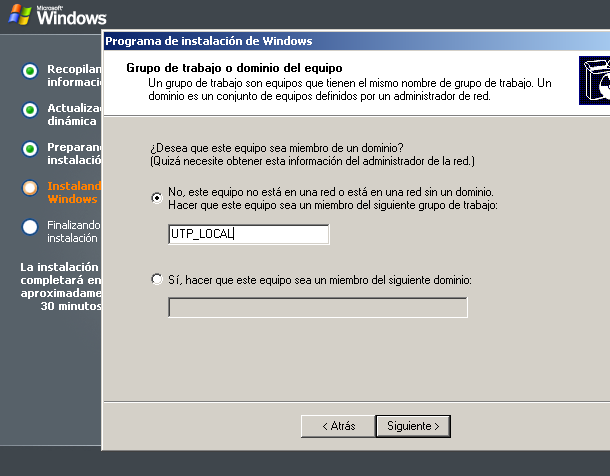
\includegraphics[width=0.68\textwidth]{imgs/20.png}
        }}
	\caption{Proceso Install Wizard}
\end{figure}

\begin{figure}[H]
 	\centering
   	\subfloat[Windows Server Configuración inicial]{\label{fig:bienvenida}{
   		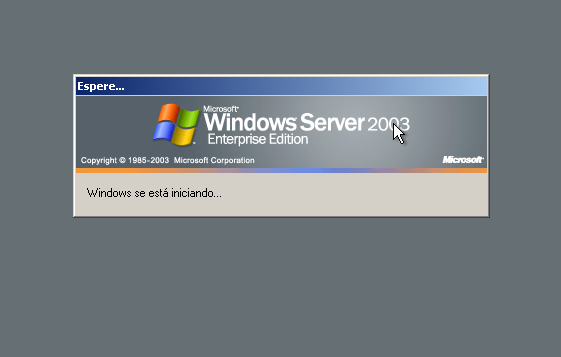
\includegraphics[width=0.68\textwidth]{imgs/21.png}
   		}}
	\subfloat[Instalacion de Guest Additions VirtualBox, drivers]{\label{fig:insta1}{
   		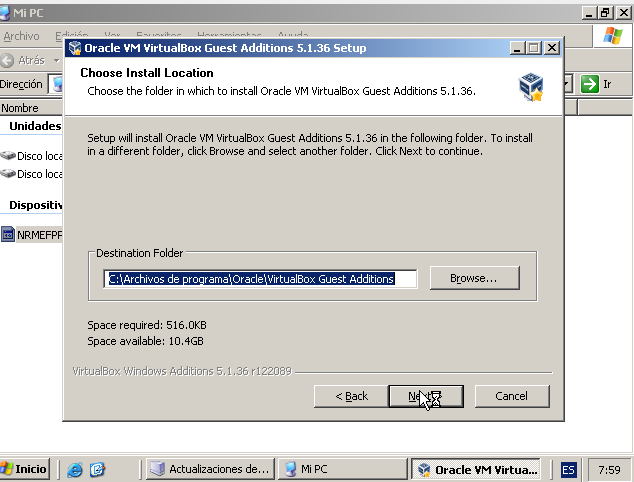
\includegraphics[width=0.68\textwidth]{imgs/22.png}
        }}
       \hfill
	\subfloat[Administrador, trabajo completo]{\label{fig:insta}{
   		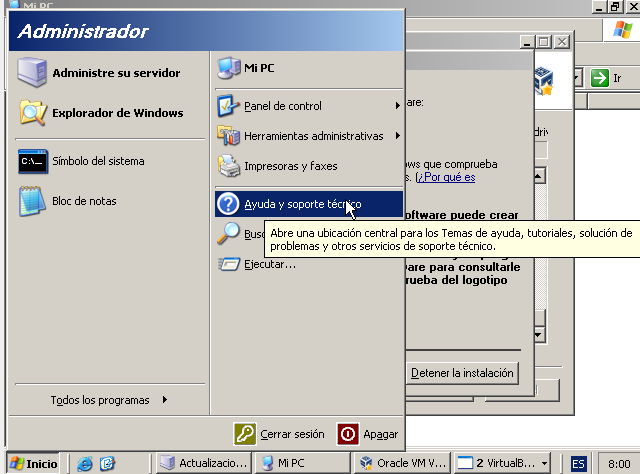
\includegraphics[width=0.68\textwidth]{imgs/23.png}
        }}
      \subfloat[Por defecto, no hay autologin en el servidor.]{\label{fig:ufs}{
   		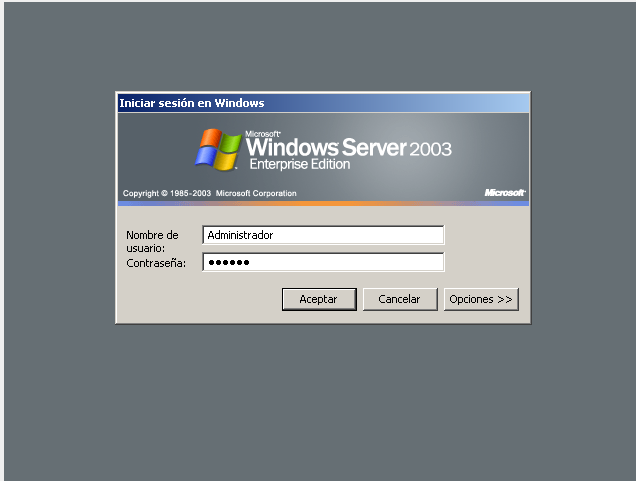
\includegraphics[width=0.68\textwidth]{imgs/24.png}
        }}
\end{figure}
Como se puede ver en las imágenes previas, la instalación del windows server se realiza de la misma manera que se realizaría un Windows XP SP3, por defecto Windows Server 2003 tiene un montón de caracteristicas des habilitados con la filosofía menos es mas, solo se realiza la instalación de los servicios y software necesario dentro del servidor. para simular la presión de las teclas ctrl + alt + supr se utiliza el teclado de virtualbox.

\newpage
\section{Proceso de instalación Directorio Activo}
\begin{center}
\begin{figure}[H]
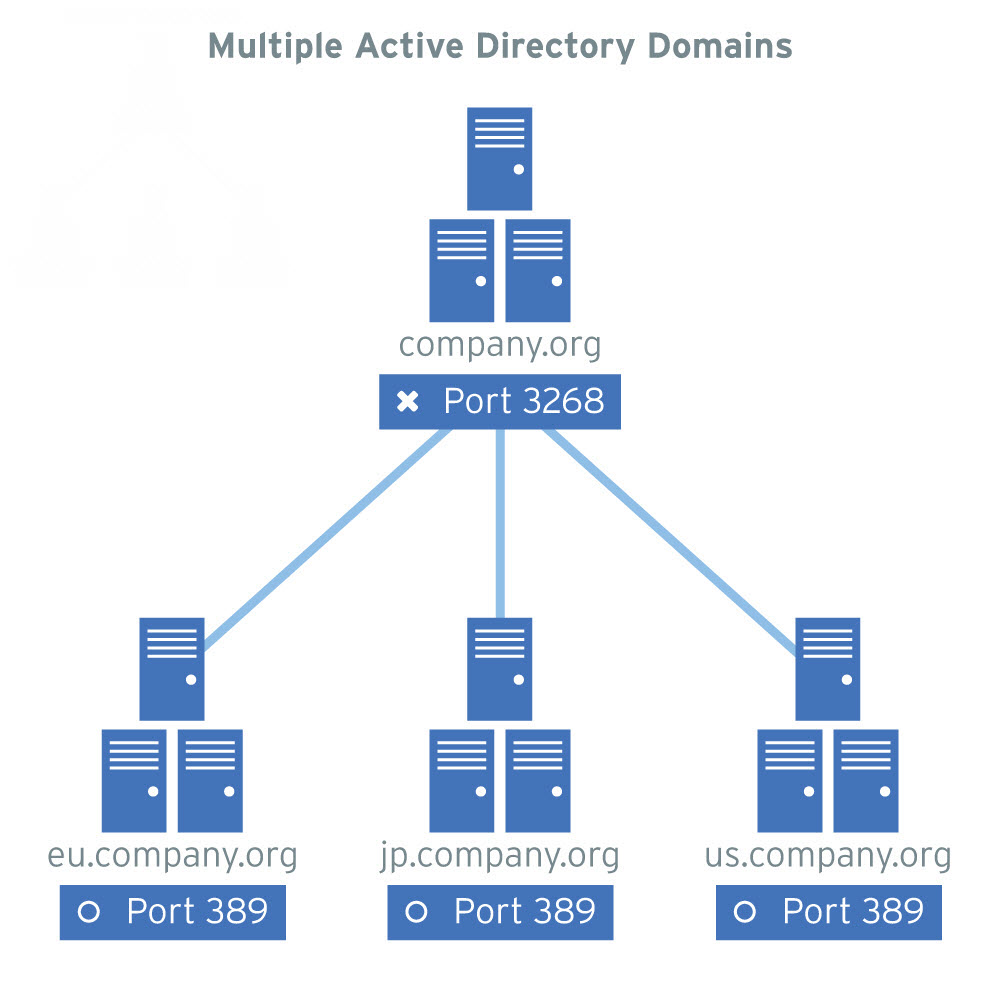
\includegraphics[scale=0.4]{imgs/acd.jpg}
\caption{Ejemplo directorio activo, company.org}
\label{fig:acd}
\end{figure}
\end{center}

El servicio de directorio de Active Directory® se puede instalar en servidores que ejecuten Microsoft® Windows Server™ 2003, Standard Edition, Windows Server 2003, Enterprise Edition y Windows Server 2003, Datacenter Edition. Active Directory almacena información sobre los objetos de la red y facilita la búsqueda y utilización de esta información para los usuarios y administradores. Active Directory utiliza un almacén de datos estructurado como base para una organización lógica y jerárquica de la información del directorio.
$$\\$$
Este almacén de datos, también denominado directorio, contiene información sobre los objetos de Active Directory. Estos objetos suelen incluir recursos compartidos como servidores, volúmenes, impresoras, cuentas de usuario de red y cuentas de equipo. Para obtener más información acerca del almacén de datos de Active Directory, vea Almacén de datos del directorio. La administración basada en directivas facilita la tarea del administrador incluso en las redes más complejas. Para obtener más información acerca de Active Directory, vea Introducción a la seguridad.

Active Directory también incluye:
\begin{itemize}
\item Un conjunto de reglas, el esquema, que define las clases de objetos y los atributos que contiene el directorio, así como las restricciones y los límites en las instancias de estos objetos y el formato de sus nombres. Para obtener más información acerca del esquema, vea Schema.
\item Un catálogo global que contiene información acerca de cada uno de los objetos del directorio. Esto permite a los usuarios y administradores encontrar información del directorio con independencia de cuál sea el dominio del directorio que realmente contiene los datos. Para obtener más información acerca del catálogo global, vea Función del catálogo global.
\item Un sistema de índices y consultas, para que los usuarios o las aplicaciones de red puedan publicar y encontrar los objetos y sus propiedades. Para obtener más información acerca de cómo realizar consultas en el directorio, vea Buscar información del directorio.
\item Un servicio de replicación que distribuye los datos del directorio por toda la red. Todos los controladores de un dominio participan en la replicación y contienen una copia completa de toda la información del directorio para su dominio. Cualquier cambio en los datos del directorio se replica en todos los controladores del dominio. Para obtener más información acerca de la replicación de Active Directory, vea Introducción a la replicación.
\item Compatibilidad con el software de cliente de Active Directory, lo que permite que muchas de las características de Microsoft® Windows® 2000 Professional o Windows XP Professional también estén disponibles en los equipos que ejecutan Windows 95, Windows 98 y NT® Server 4.0. En los equipos que no ejecutan el software de cliente de Active Directory, el directorio tendrá el mismo aspecto que un directorio de Windows NT. Para obtener más información acerca del software de cliente, vea Clientes de Active Directory.
\end{itemize}

Para realizar su instalación solo se debe utilizar el install wizard que provee o habilitar el servicio desde el panel caracteristicas de windows.

A continuación se detalla el proceso. 

\begin{figure}[H]
 	\centering
   	\subfloat[Iniciamos sesion en el servidor]{\label{fig:bienvenida}{
   		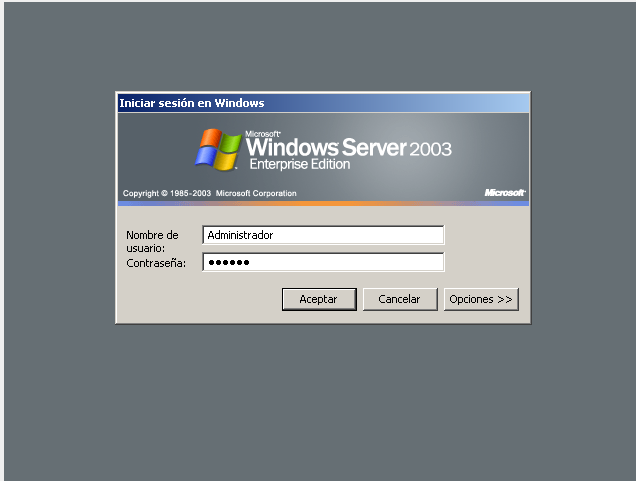
\includegraphics[width=0.68\textwidth]{imgs/24.png}
   		}}
	\subfloat[Utilizamos el asisten rapido de configuracion, seleccionando Servidor directorio activo]{\label{fig:insta1}{
   		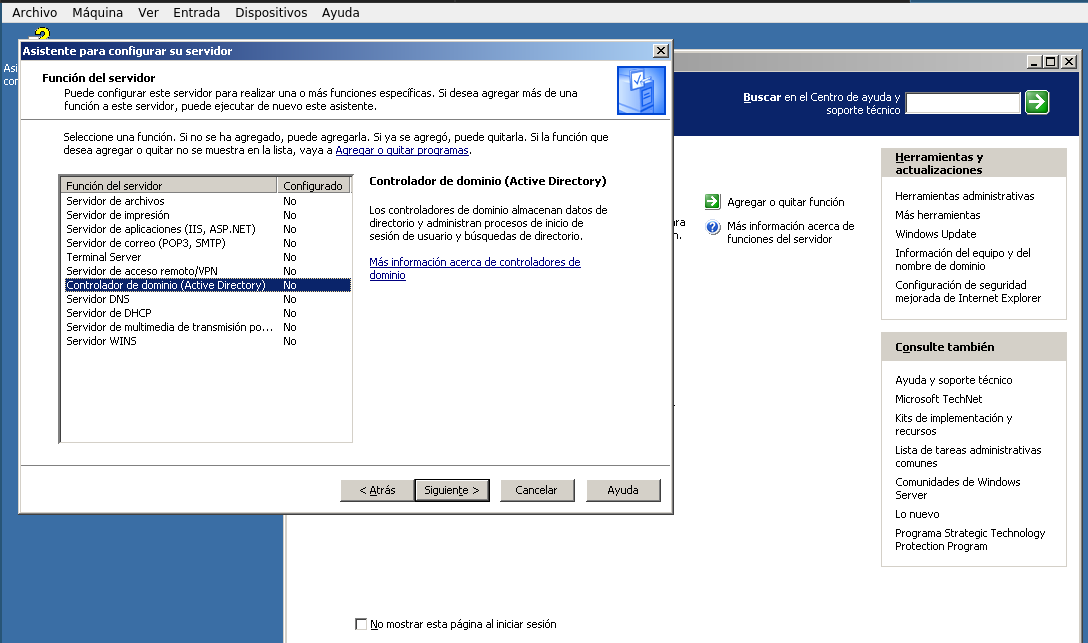
\includegraphics[width=0.68\textwidth]{imgs/25.png}
        }}
       \hfill
	\subfloat[Controlador de Dominio]{\label{fig:insta}{
   		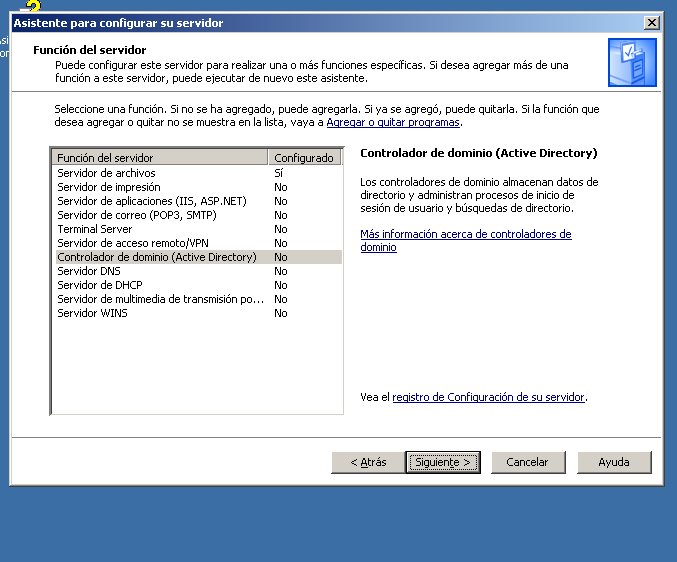
\includegraphics[width=0.68\textwidth]{imgs/26.png}
        }}
      \subfloat[Install Wizard.]{\label{fig:ufs}{
   		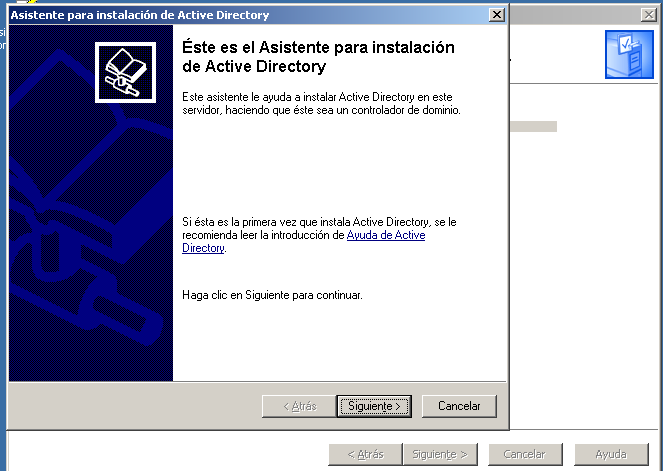
\includegraphics[width=0.68\textwidth]{imgs/27.png}
        }}
        \hfill
	\subfloat[Opcion de dominio nuevo]{\label{fig:inicianbase}{
   		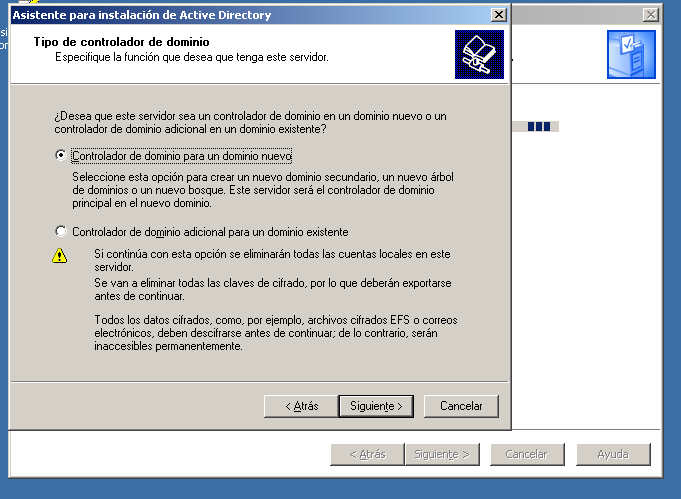
\includegraphics[width=0.68\textwidth]{imgs/28.png}
        }}
      \subfloat[Nombre de dns]{\label{fig:ufs}{
   		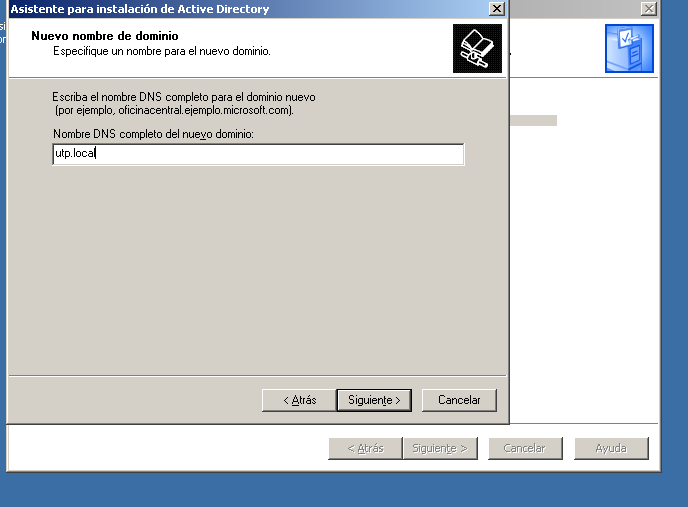
\includegraphics[width=0.68\textwidth]{imgs/29.png}
        }}
	\caption{Proceso de Instalacion Windows Server}
\end{figure}

\begin{figure}[H]
 	\centering
   	\subfloat[Ubicacion de Base de datos]{\label{fig:bienvenida}{
   		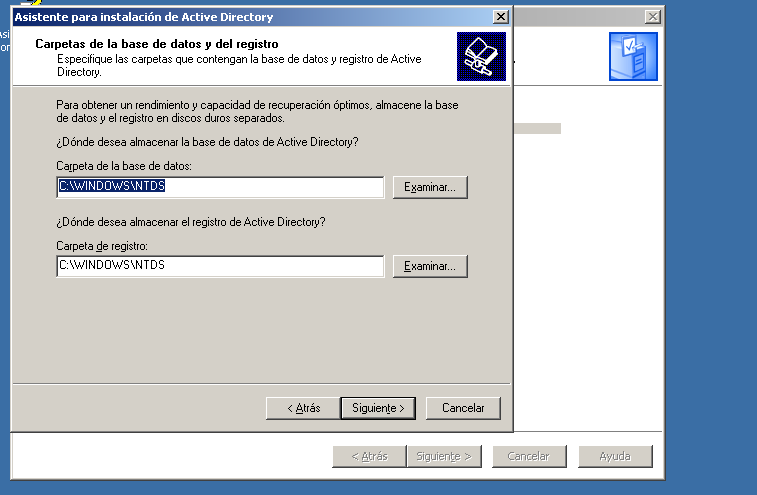
\includegraphics[width=0.68\textwidth]{imgs/30.png}
   		}}
	\subfloat[compatibilidad de permisos en todo el controlador los permisos son heredados a partir de una política de seguridad.]{\label{fig:insta1}{
   		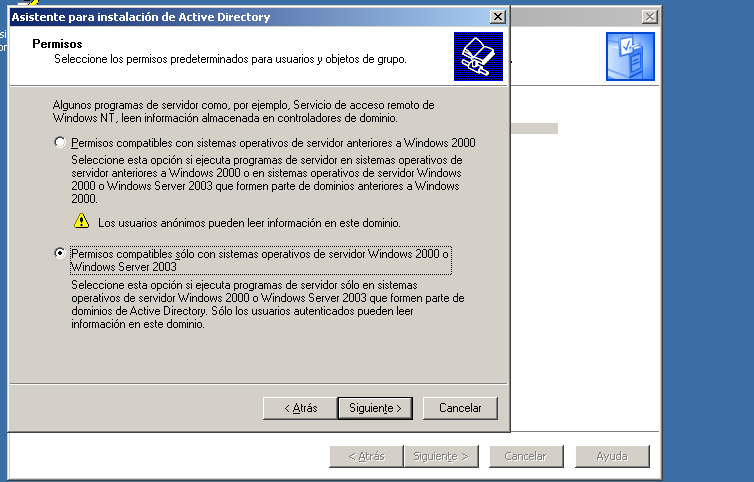
\includegraphics[width=0.68\textwidth]{imgs/31.png}
        }}
       \hfill
	\subfloat[Progreso de instalación, despliegue]{\label{fig:insta}{
   		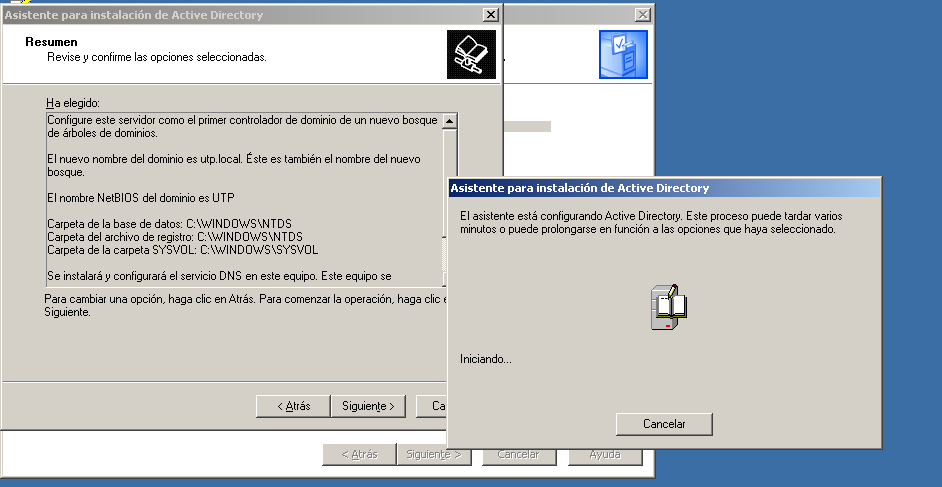
\includegraphics[width=0.68\textwidth]{imgs/32.png}
        }}
      \subfloat[Proceso Finalizado.]{\label{fig:ufs}{
   		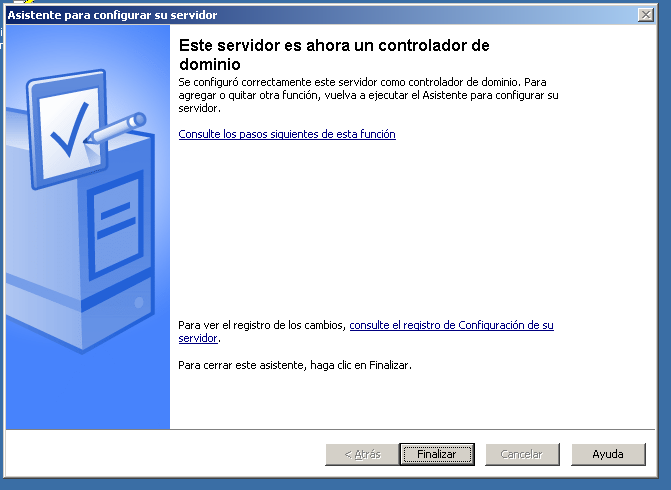
\includegraphics[width=0.68\textwidth]{imgs/33.png}
        }}
	\caption{Proceso secuencial de instalación, Active Directory}
\end{figure}

\section{Manejo de Archivos}
Windows Server 2003 viene por defecto con el Explorador de Windows, este es el administrador de archivos oficial del sistema operativo Microsoft Windows.
\begin{center}
\begin{figure}[H]
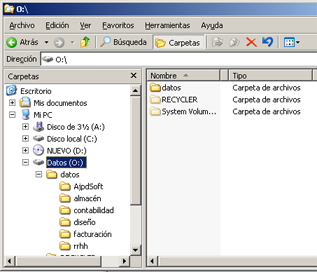
\includegraphics[]{imgs/explorer.png}
\caption{Explorador de Windows}
\label{fig:files}
\end{figure}
\end{center}

El explorador viene con las siguientes caracteristicas : 

\textbf{Explorer}: modo de gestión espacial, cada carpeta se abrirá en una ventana separada. Los tamaños se fijan automáticamente según el contenido de la carpeta nuevamente abierta. Por ejemplo, una carpeta con dos archivos se abre con una ventana más pequeña que el de una carpeta con diez archivos. Además, cuando hay centenares de archivos en una carpeta, la carpeta se presentará automáticamente en modo de "lista".
Con Windows 98, parte del código de Internet Explorer, fue añadido al Explorador; como por ejemplo la barra de direcciones para ver páginas web. 

Barra de tareas en vez del árbol de carpetas, con acciones comunes relativas al archivo seleccionado; selecciona otros lugares, tales como "MI PC", "Panel de control", y "Mis documentos". Estos también cambian dependiendo de qué archivo se trata, pero no se puede definir accesos a otras carpetas o información adicional (tamaño y fecha del archivo, tipo, autor, dimensiones de la imagen, y otros detalles).

Pre visualización de imágenes, con soporte de Exif y envío de correos electrónicos.

Soporte FTP, aunque esta capacidad está muy limitada si lo comparamos con apps dedicadas como Filezilla.

Capacidad nativa para grabar imágenes de CD-DVD, disponible en las versiones Professional y Enterprise de Windows XP,  WIndows Server 2003.

\section{Estructura del Sistema Operativo}
La información del diseño del sistema operativo la obtengo de \fnurl{aqui}{https://tutorialx.wordpress.com/2009/10/06/tutoriale-online-windows-server-2003-structural-modes-subsystem-and-managers/}
Basicamente este sistema operativo al igual que los demás que hemos observado funcionan en dos posibles modos.
\begin{itemize}
\item Modo privilegiado, kernel o modo ejecutivo
\item Modo usuario, no privilegiado
\end{itemize}

En el primer modo el sistema operativo administra servicios, datos de sistema, interfaces de red que son controlados por el kernel.

En el modo usuario, corre lo demas en este caso en Subsystema Win32 Y otros subsistemas que interaccionan con el usuario atravez de una API integrada para el manejo de hardware y datos.
\begin{center}
\begin{figure}[H]
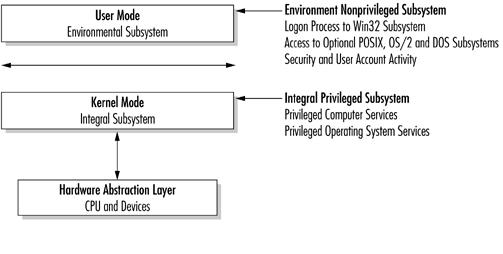
\includegraphics[scale=0.98]{imgs/kernelmodes.jpg}
\caption{Modos de ejecucion, Windows Server 2003.}
\label{fig:mejora}
\end{figure}
\end{center}
\subsubsection{Modo ejecutivo}
El modo ejecutivo de Windows Server 2003 es tambien conocido como el modo privilegiado. Windows Server 2003 divide la operacion en 5 secciones: 
\begin{enumerate}
\item Hardware abstraction layer (HAL)
\item Microkernel
\item Device drivers
\item Executive managers
\item Executive services buffer
\end{enumerate}
como se observa en la figura \ref{fig:kernel}
\begin{center}
\begin{figure}[H]
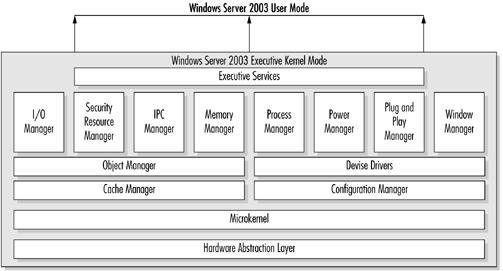
\includegraphics[scale=0.9]{imgs/kernel.jpg}
\caption{Timeline, Microsoft Windows. Sistemas Operativos y relación de Kernels}
\label{fig:kernel}
\end{figure}
\end{center}
Colectiva mente estos elementos maneja las responsabilidades del sistema que son transparentes a el usuario. En Windows Server 2003, el modo ejecutivo controla las funciones esenciales para el funcionamiento del sistema operativo. Otras funciones son puestas en el modo no protegido. Todos los 5 elementos son independientes entre si e intercambian datos a través de API, y mensajes correspondientes. En teoría cualquier componente de los 5 puede ser eliminado y reemplazado tecnológicamente.
\newpage
\section{Clasificación}
Este sistema operativo se clasifica como :
\begin{enumerate}
\item Multiusuario:  Permite multiples inicios de session en la misma maquina. 
\item Multitareas: Es posible realizar multiples actividades en la misma maquina al tiempo.
\item Propósito general, pues se puede dedicar el servidor a cualquier  uso desde servidor de impresiones hasta servidor web.
\item máquina virtual.
\item cerrado. 
\end{enumerate}

\end{document}